\documentclass[aspectratio=169]{beamer}
\usepackage[english]{babel}
\usepackage[T1]{fontenc}
\usepackage[utf8]{inputenc}
\usepackage{graphicx}
\graphicspath{
        {../}
}

\usepackage{listings}
% Source Code
\usepackage{color}

\mode<presentation>
{
  \usetheme{default}

  \setbeamercovered{transparent}

  % Frame titles (inherits from titlelike)
  \setbeamerfont{frametitle}{size=\LARGE}

  % Top-level itemize items are prefixed with a square
  \setbeamertemplate{itemize item}[square]
  % Top-level enumerate items are *not* in a shape
  \setbeamertemplate{enumerate items}[default]
  % Subitems are prefixed with a triangle
  \setbeamertemplate{itemize subitem}[triangle]
}

\AtBeginSection[]{%
  \begin{frame}
    \vfill
    \centering
    {\usebeamerfont{title}\insertsectionhead\par}
    \vfill
  \end{frame}
}

\newcommand{\myCommentStyle}[1]{{\footnotesize\ttfamily\color{gray!100!white} #1}}
% my string style
\newcommand{\myStringStyle}[1]{{\footnotesize\ttfamily\color{violet!100!black} #1}}
% my symbol style
\newcommand{\mySymbolStyle}[1]{{\footnotesize\ttfamily\color{violet!100!black} #1}}
% my keyword style
\newcommand{\myKeywordStyle}[1]{{\footnotesize\ttfamily\color{green!70!black} #1}}

\lstset{
language={},
tabsize=3,
escapechar={!},
keepspaces=true,
breaklines=true,
alsoletter={\#},
literate={\$}{{{\$}}}1,
breakautoindent=true,
columns=fullflexible,
showstringspaces=false,
frame=single,
aboveskip=1em, % automatic space before
framerule=0pt,
basicstyle=\ttfamily\color{black},
keywordstyle=\myKeywordStyle,% keyword style
commentstyle=\myCommentStyle,% comment style
frame=single,%
stepnumber=1,
numbersep=10pt,
numberstyle=\tiny,
numberfirstline=true,
captionpos=b,
moredelim=[is][\bfseries]{&lt;b&gt;}{&lt;/b&gt;},
moredelim=[is][\textit]{&lt;i&gt;}{&lt;/i&gt;},
moredelim=[is][\underbar]{&lt;u&gt;}{&lt;/u&gt;},
moredelim=[is][\color{red}\uwave]{&lt;wave&gt;}{&lt;/wave&gt;},
moredelim=[is][\color{red}\sout]{&lt;del&gt;}{&lt;/del&gt;},
moredelim=[is][\color{blue}\underbar]{&lt;ins&gt;}{&lt;/ins&gt;},
morecomment=[s][\myCommentStyle]{"}{"},
morestring=[b][\myStringStyle]',
moredelim=[is][]{&lt;sel&gt;}{&lt;/sel&gt;},
moredelim=[is][]{&lt;rcv&gt;}{&lt;/rcv&gt;},
moredelim=[is][\itshape]{&lt;symb&gt;}{&lt;/symb&gt;},
moredelim=[is][\scshape]{&lt;class&gt;}{&lt;/class&gt;},
morekeywords={true,false,nil,self,super,thisContext},
identifierstyle=\idstyle,
}

\lstdefinelanguage{diff}{
  sensitive=true,
  % diff command line
  morecomment=[f][\color{gray}][0]{diff},
  % commit identifiers for git diff
  morecomment=[f][\color{gray}][0]{index},
  % hunk location/line numbers for unified format
  morecomment=[f][\color{blue}][0]{@@},
  % hunk location/line numbers for context format
  morecomment=[f][\color{magenta}][0]{***},
  % changed line for context format
  morecomment=[f][\color{violet}][0]{!},
  % deleted lines for unified format
  morecomment=[f][\color{red!60!black}][0]-,
  % added lines for unified format
  morecomment=[f][\color{green!60!black}][0]+,
  % file name and time stamp old file
  morecomment=[f][\color{magenta}][0]{---},
  % file name and time stamp new file
  morecomment=[f][\color{magenta}][0]{+++},
  % Binary files ... differ
  morecomment=[f][\color{gray}][0]{Binary},
  % Only in ...: file.txt
  morecomment=[f][\color{gray}][0]{Only},
  % old mode ...
  morecomment=[f][\color{gray}][0]{old},
  % new mode ...
  morecomment=[f][\color{gray}][0]{new},
  % rename from/to ...
  morecomment=[f][\color{gray}][0]{rename},
  % similarity index ...%
  morecomment=[f][\color{gray}][0]{similarity},
  % deleted file mode ...%
  morecomment=[f][\color{gray}][0]{deleted},
  % hunk separator for context format
  morecomment=[f][\color{magenta}][0]{***************},
  % deleted lines for normal format
  morecomment=[f][\color{red!60!black}][0]<,
  % added lines for normal format
  morecomment=[f][\color{green!60!black}][0]>,
  % line number specifier for normal format
  morecomment=[f][\color{blue}][0]{0},
  % line number specifier for normal format
  morecomment=[f][\color{blue}][0]{1},
  % line number specifier for normal format
  morecomment=[f][\color{blue}][0]{2},
  % line number specifier for normal format
  morecomment=[f][\color{blue}][0]{3},
  % line number specifier for normal format
  morecomment=[f][\color{blue}][0]{4},
  % line number specifier for normal format
  morecomment=[f][\color{blue}][0]{5},
  % line number specifier for normal format
  morecomment=[f][\color{blue}][0]{6},
  % line number specifier for normal format
  morecomment=[f][\color{blue}][0]{7},
  % line number specifier for normal format
  morecomment=[f][\color{blue}][0]{8},
  % line number specifier for normal format
  morecomment=[f][\color{blue}][0]{9},
}[comments]

\lstnewenvironment{diff}[2][defaultlabel]{%
\renewcommand{\lstlistingname}{Diff}%
        \lstset{
                % frame=lines,
                frame=single,
                framerule=0pt,
                mathescape=false,
                name={Diff},
                title={#1},
                language=diff
        }
}{}
\usepackage{fixltx2e}

%Information to be included in the title page:
\title{Griotte}
\subtitle{Code Review with Fine-Grained IDE Events}
\author{Skip Lentz, Mart\'{i}n Dias, Damien Cassou}
\institute{TU Delft, INRIA Lille - Nord Europe}
\date{December 3, 2015}

\begin{document}

\begin{frame}

\titlepage
\centering

\includegraphics[width=40mm]{img/tu_delft_logo.eps}

\includegraphics[width=40mm]{img/inria_logo.eps}
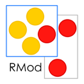
\includegraphics{img/rmod_logo.png}

\end{frame}

\begin{frame}[fragile]

\frametitle{Introduction}

\begin{itemize}
\item Intern at INRIA (RMoD) from TU Delft
\begin{itemize}
\item Mentored by Mart\'{i}n Dias and Damien Cassou at RMoD
\item Remotely co-mentored by Alberto Bachelli at TU Delft
\end{itemize}

\item Working on Code Review within Pharo
\end{itemize}
\end{frame}

\begin{frame}[fragile]

\frametitle{Outline}

\tableofcontents%

\end{frame}

\section{Problem Description}

\begin{frame}[fragile]

\frametitle{Problem Description}

\begin{columns}

\begin{column}{0.5\textwidth}

Code review is difficult:

\begin{enumerate}
\item<1-> Tangled commits
\item<2-> Line-based view
\item<3-> Shadowed changes
\item<4-> Bad commit descriptions
\end{enumerate}
\end{column}

\begin{column}{0.5\textwidth}

\begin{onlyenv}<1>
  Two concerns, one commit:
\begin{diff}[Example~(Jaxen@08b4f72)]

   *
-  */public interface AdditiveExpr extends BinaryExpr
+  */
+ public interface AdditiveExpr extends BinaryExpr
  {
-     String getOperator();
  }
\end{diff}
\end{onlyenv}

\begin{onlyenv}<2>
  Scattered changes:
\begin{diff}[File A.java]

- public static void bar() {
+ public static void foo() {
\end{diff}
\begin{diff}[File B.java]

- A.bar();
+ A.foo();
\end{diff}
\begin{diff}[File C.java]

- A.bar();
+ A.foo();
\end{diff}
\end{onlyenv}

\begin{onlyenv}<3>
  For example:
  \begin{enumerate}
  \item method \texttt{foo}: First try for bug fix.
  \item test run: Tests fail.
  \item method \texttt{foo}: Debug and try again.
  \item test run: Tests succeed.
  \end{enumerate}
  The first change to \texttt{foo} is \textit{shadowed}.
\end{onlyenv}

\begin{onlyenv}<4>
  Commit messages:
  \begin{itemize}
  \item "Fix bug"
  \item "Some changes"
  \end{itemize}
\end{onlyenv}

\end{column}

\end{columns}

\end{frame}

\section{Proposed Solution}

\begin{frame}[fragile]

\frametitle{Fine-Grained IDE Events}

\begin{columns}

\begin{column}{0.5\textwidth}

\begin{itemize}
\item Events monitored as they happen in IDE
\item Stored in a log
\item PhD thesis by Mart\'{i}n~Dias
\end{itemize}
\end{column}

\begin{column}{0.5\textwidth}

\begin{figure}
\begin{center}
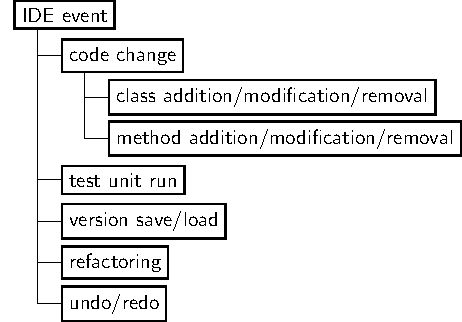
\includegraphics[width=0.9\textwidth]{img/events_model_diagram.pdf}
\end{center}
\caption{Events class hierarchy}
\end{figure}

\end{column}

\end{columns}

\end{frame}

\begin{frame}[fragile]

\frametitle{Code Review w/ Fine-Grained IDE Events}

\begin{columns}

\begin{column}{0.5\textwidth}

Use the fine-grained IDE events in code review:

\begin{itemize}
\item<1-> Display fine-grained history to the reviewer
\item<2-> Group changes together
\begin{itemize}
\item<2-> Description generated by fine-grained information
\end{itemize}

\end{itemize}
\end{column}

\begin{column}{0.5\textwidth}

\begin{onlyenv}<1>
\begin{figure}
\begin{center}
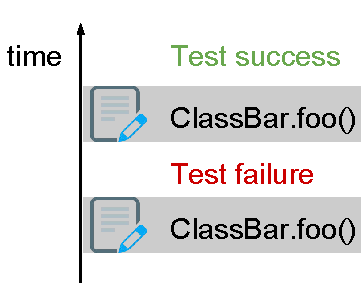
\includegraphics[width=0.9\textwidth]{img/example_log.pdf}
\end{center}
\caption{Example log}
\end{figure}
\end{onlyenv}

\begin{onlyenv}<2>
\begin{figure}
\begin{center}
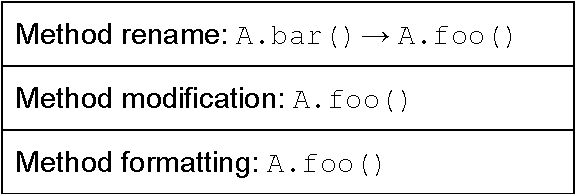
\includegraphics[width=0.9\textwidth]{img/example_groups.pdf}
\end{center}
\caption{Grouped changes}
\end{figure}
\end{onlyenv}

\end{column}

\end{columns}

\end{frame}

\section{Implementation}

\begin{frame}[fragile]

\frametitle{Implementation: Griotte}

Code review tool in Pharo.

Key ideas:

\begin{itemize}
\item Epicea as a source for fine-grained IDE events
\item Uses existing services (e.g. GitHub, Gerrit)
\end{itemize}
\end{frame}

\section{Questions/Discussion}

\end{document}

%%% Local Variables:
%%% mode: latex
%%% TeX-master: t
%%% End:
